\section{Versuchsanordnung und -durchführung}

\subsection{Versuchsaufbau}

Der Aufbau dieses Versuchs ist in Abbildung \ref{schaltung} schematisch dargestellt und besteht aus zwei NaJ-Detektoren, drei verschiedenen Strahlungsquellen, der signalverarbeitenden Elektronik sowie einem Computer.
\begin{figure}[H]
	\centering
	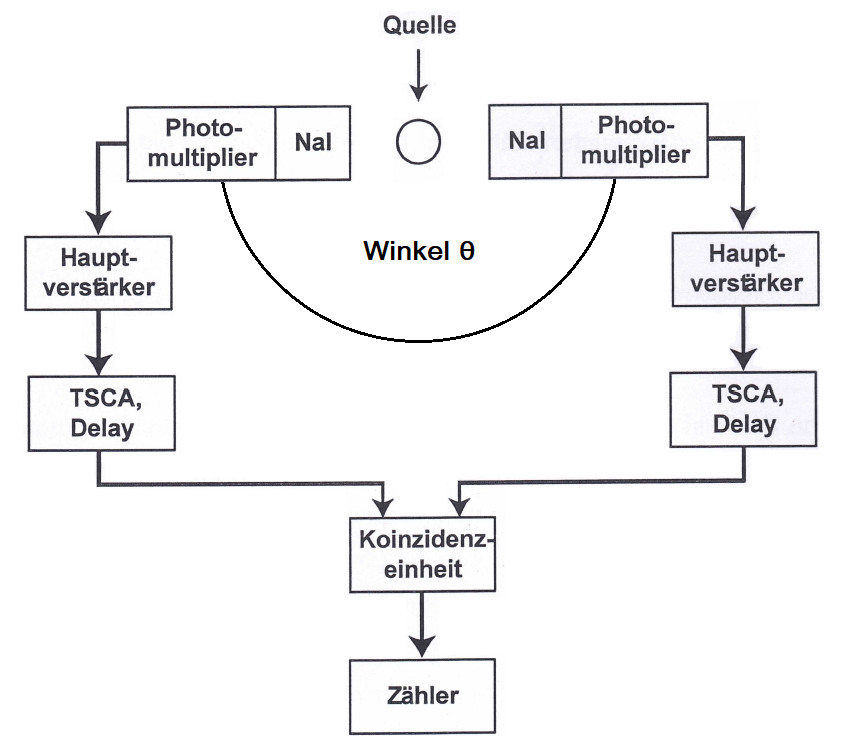
\includegraphics[width=1.0\textwidth]{img/schaltung}
	\caption{In dieser Abbildung ist der schematische Aufbau dieses Versuchs in Form eines Blockschaltbilds dargestellt. Die Abbildung wurde der Seite 15 der Versuchsanleitung\cite{wwu} entnommen und anschließend bearbeitet.}
	\label{schaltung}
\end{figure}
\noindent Bei den drei Strahlungsquellen handelt es sich um Natrium-$22$ ($^{22}$Na), Caesium-$137$ ($^{137}$Cs) und Cobalt-$60$ ($^{60}$Co).
Deren Zerfallsschemata sind in Abbildung \ref{Zerfallsschemata} zu sehen.
\begin{figure}[H]
	\centering
	\begin{subfigure}[t]{0.5\textwidth}
		\centering
		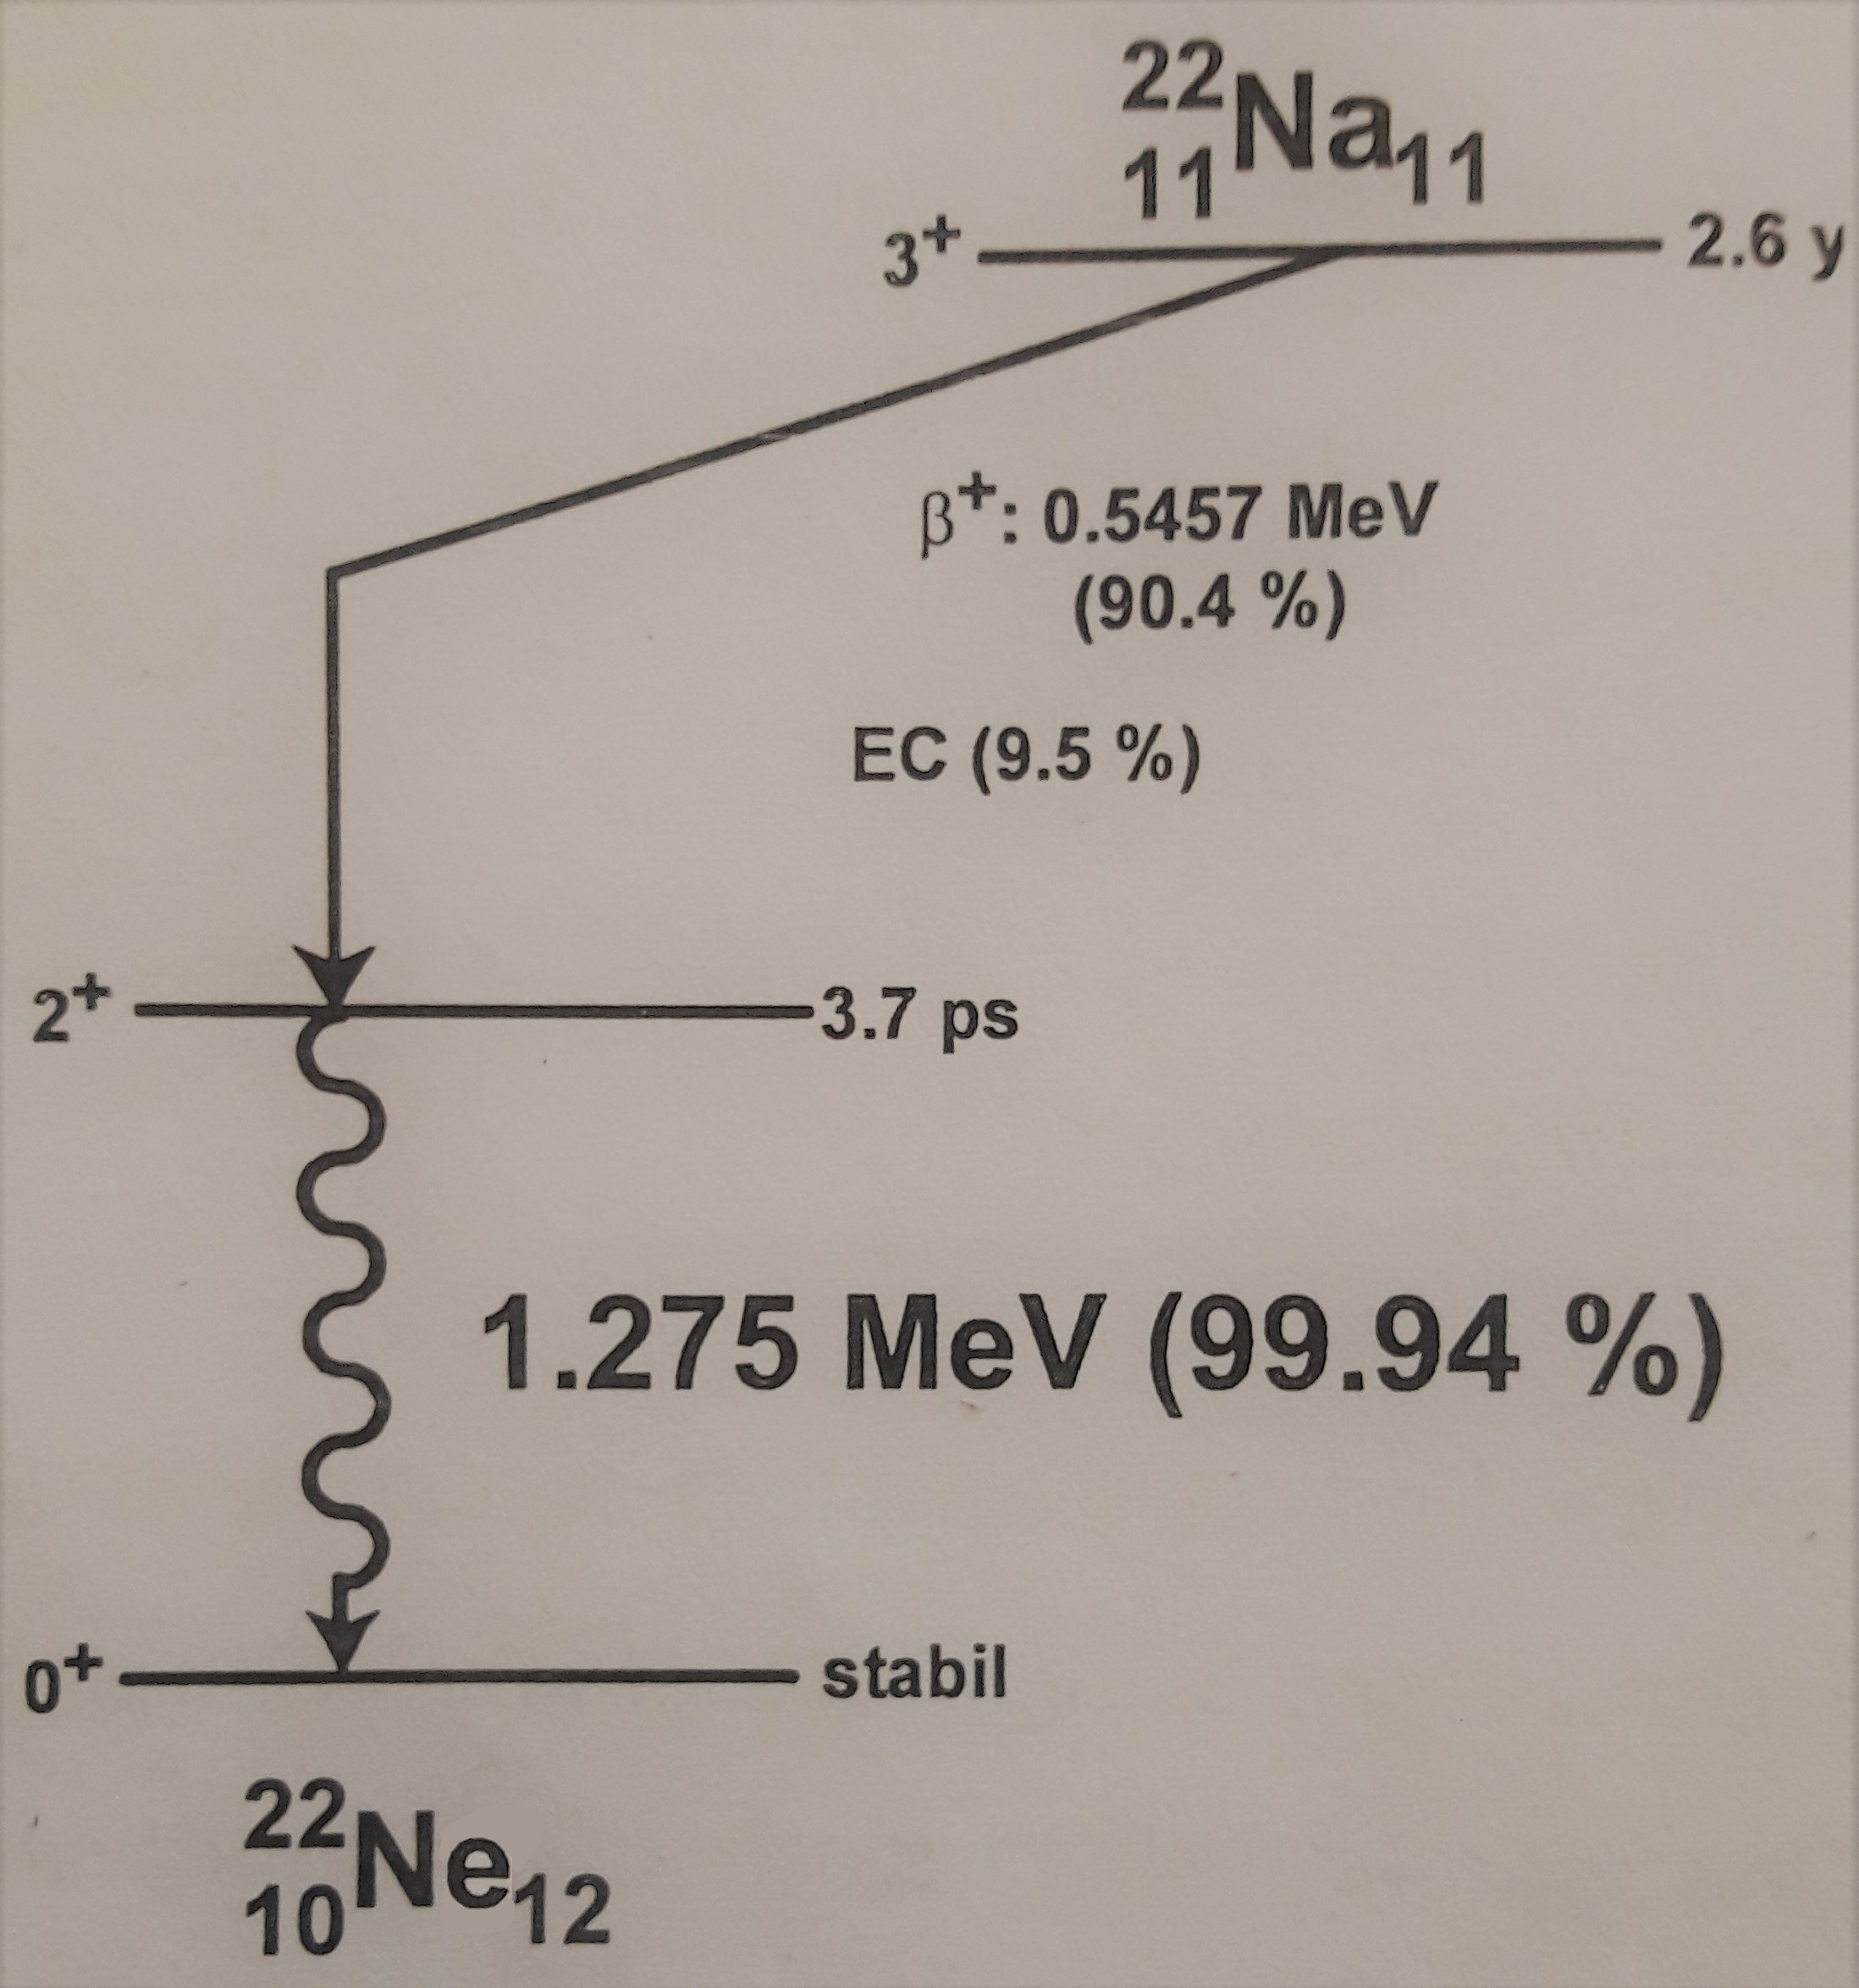
\includegraphics[width=\textwidth]{img/ZerfallsschemaVonNa22}
		\caption{Zerfallsschema von $^{22}$Na.}
	\end{subfigure}
	\begin{subfigure}[t]{0.5\textwidth}
		\centering
		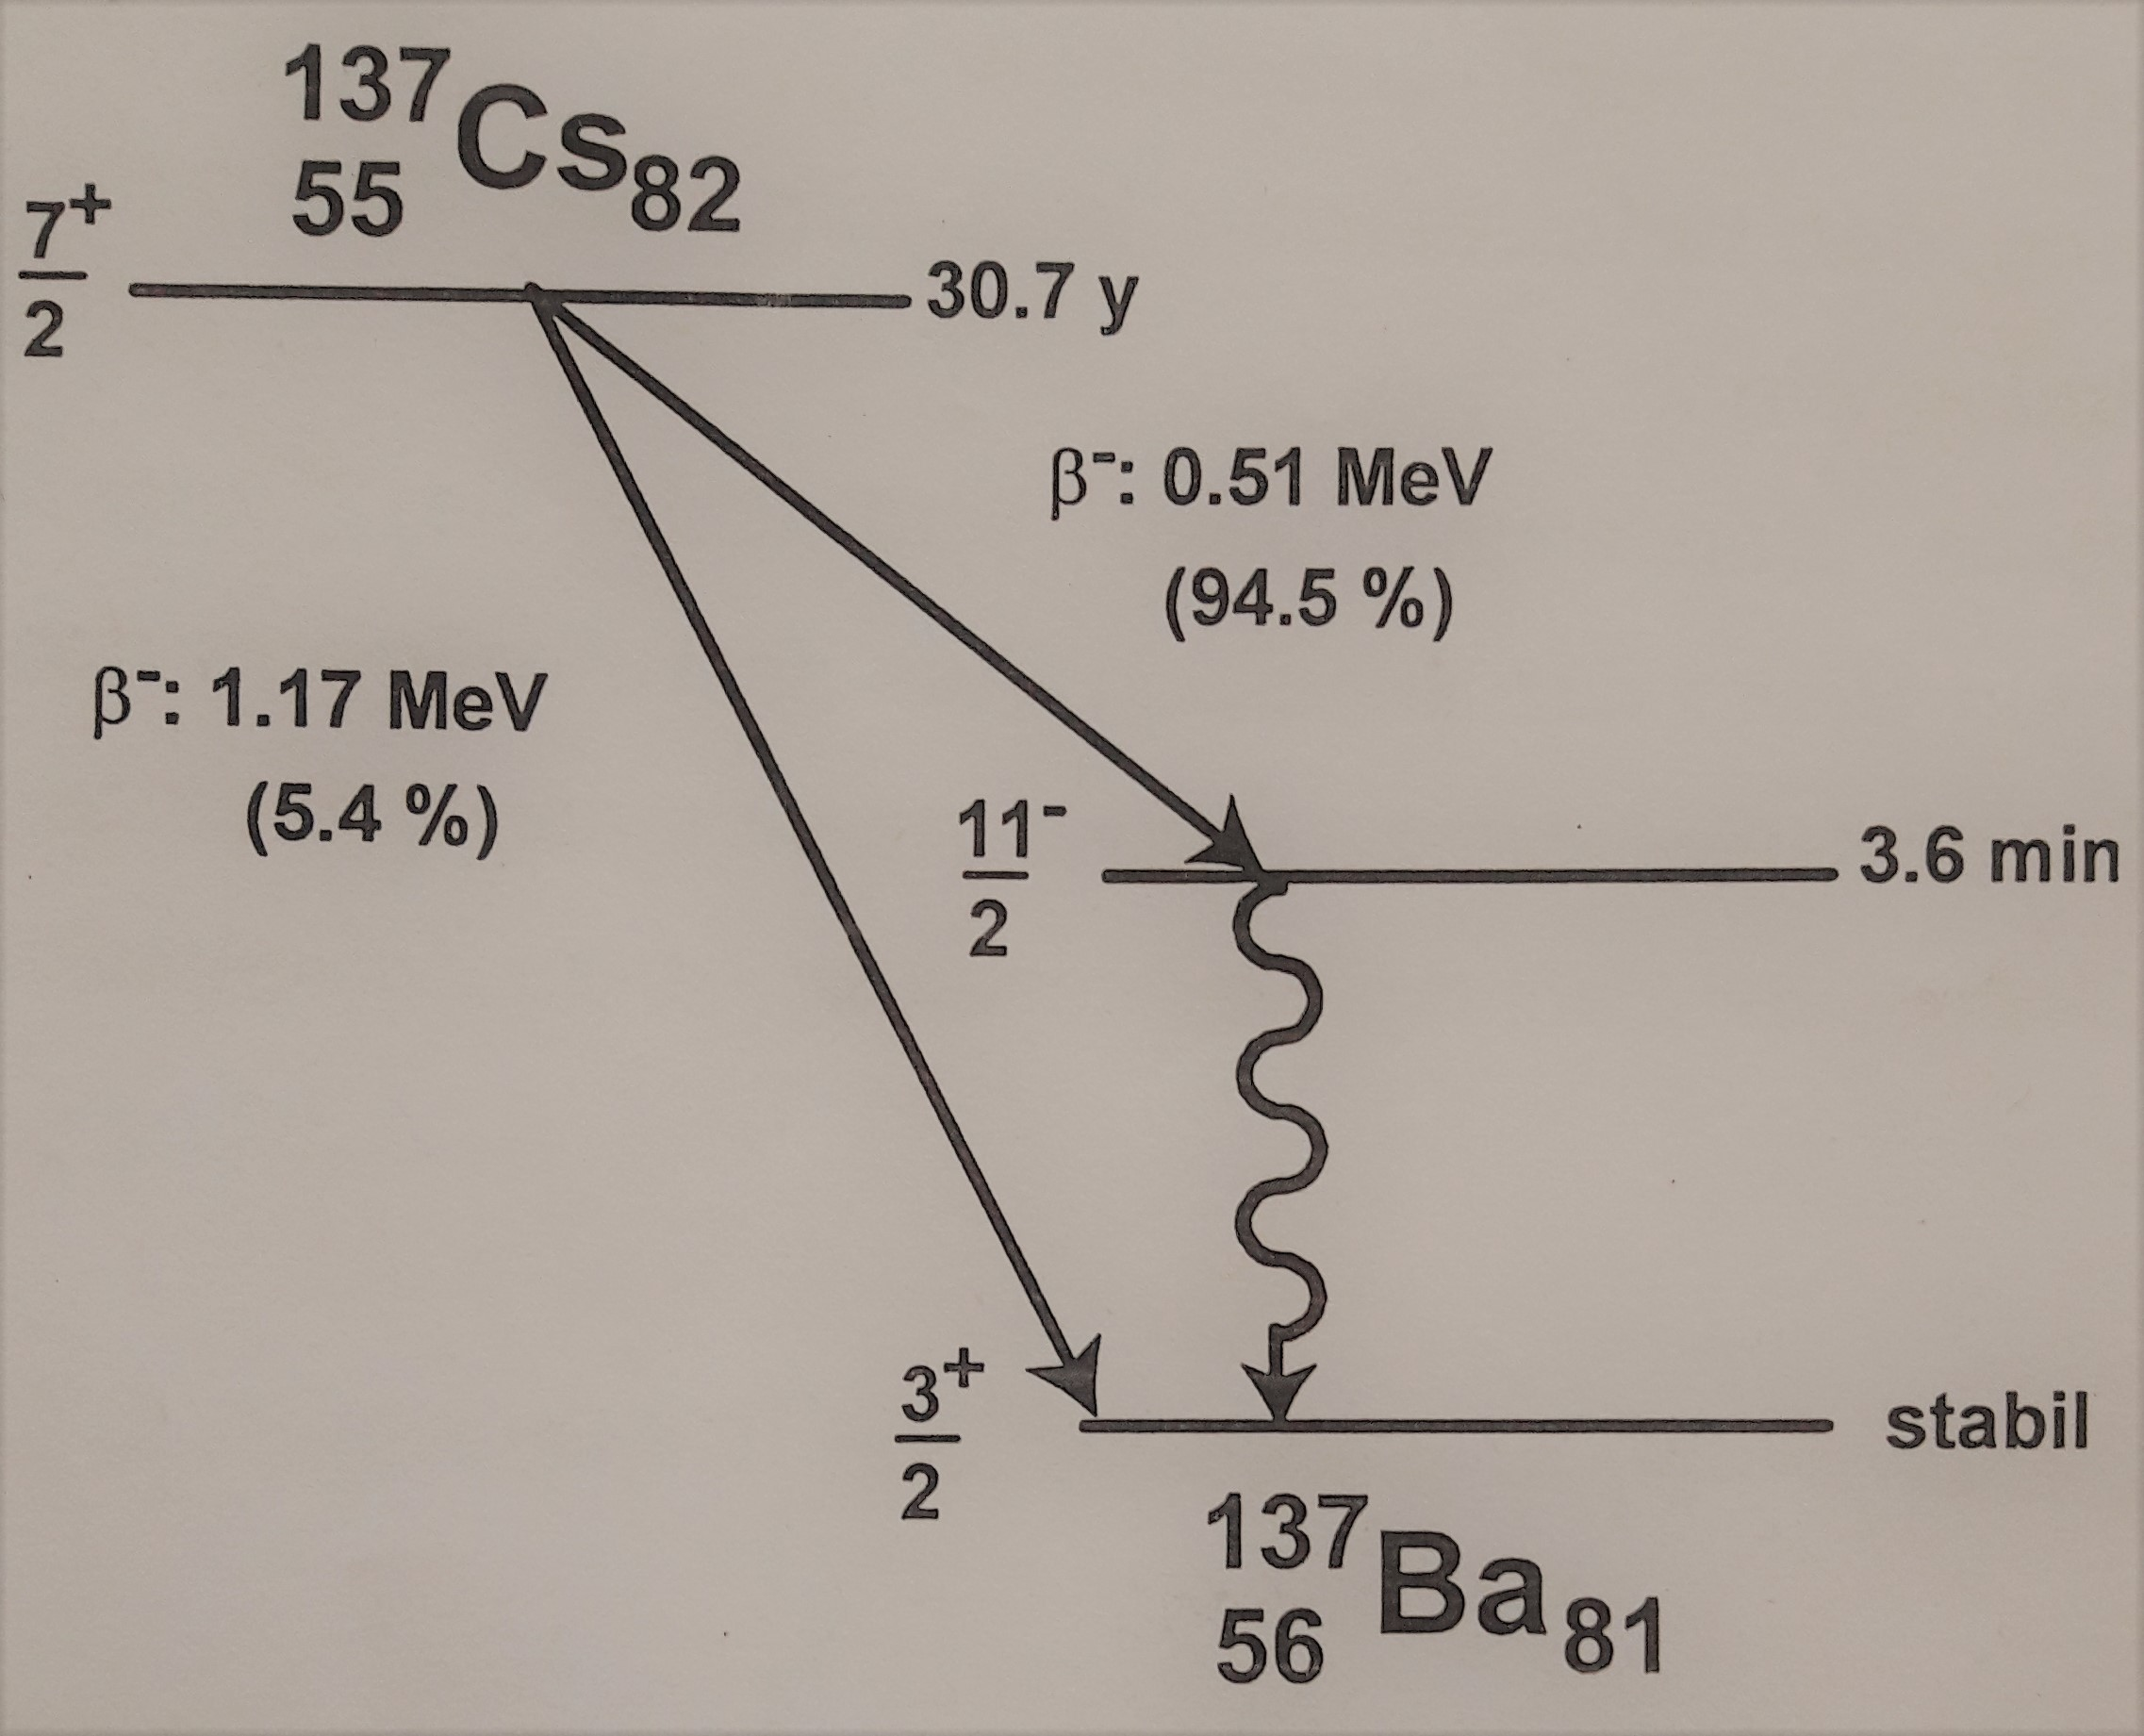
\includegraphics[width=\textwidth]{img/ZerfallsschemaVonCs137}
		\caption{Zerfallsschema von $^{137}$Cs.}
	\end{subfigure}
	\begin{subfigure}[t]{0.5\textwidth}
		\centering
		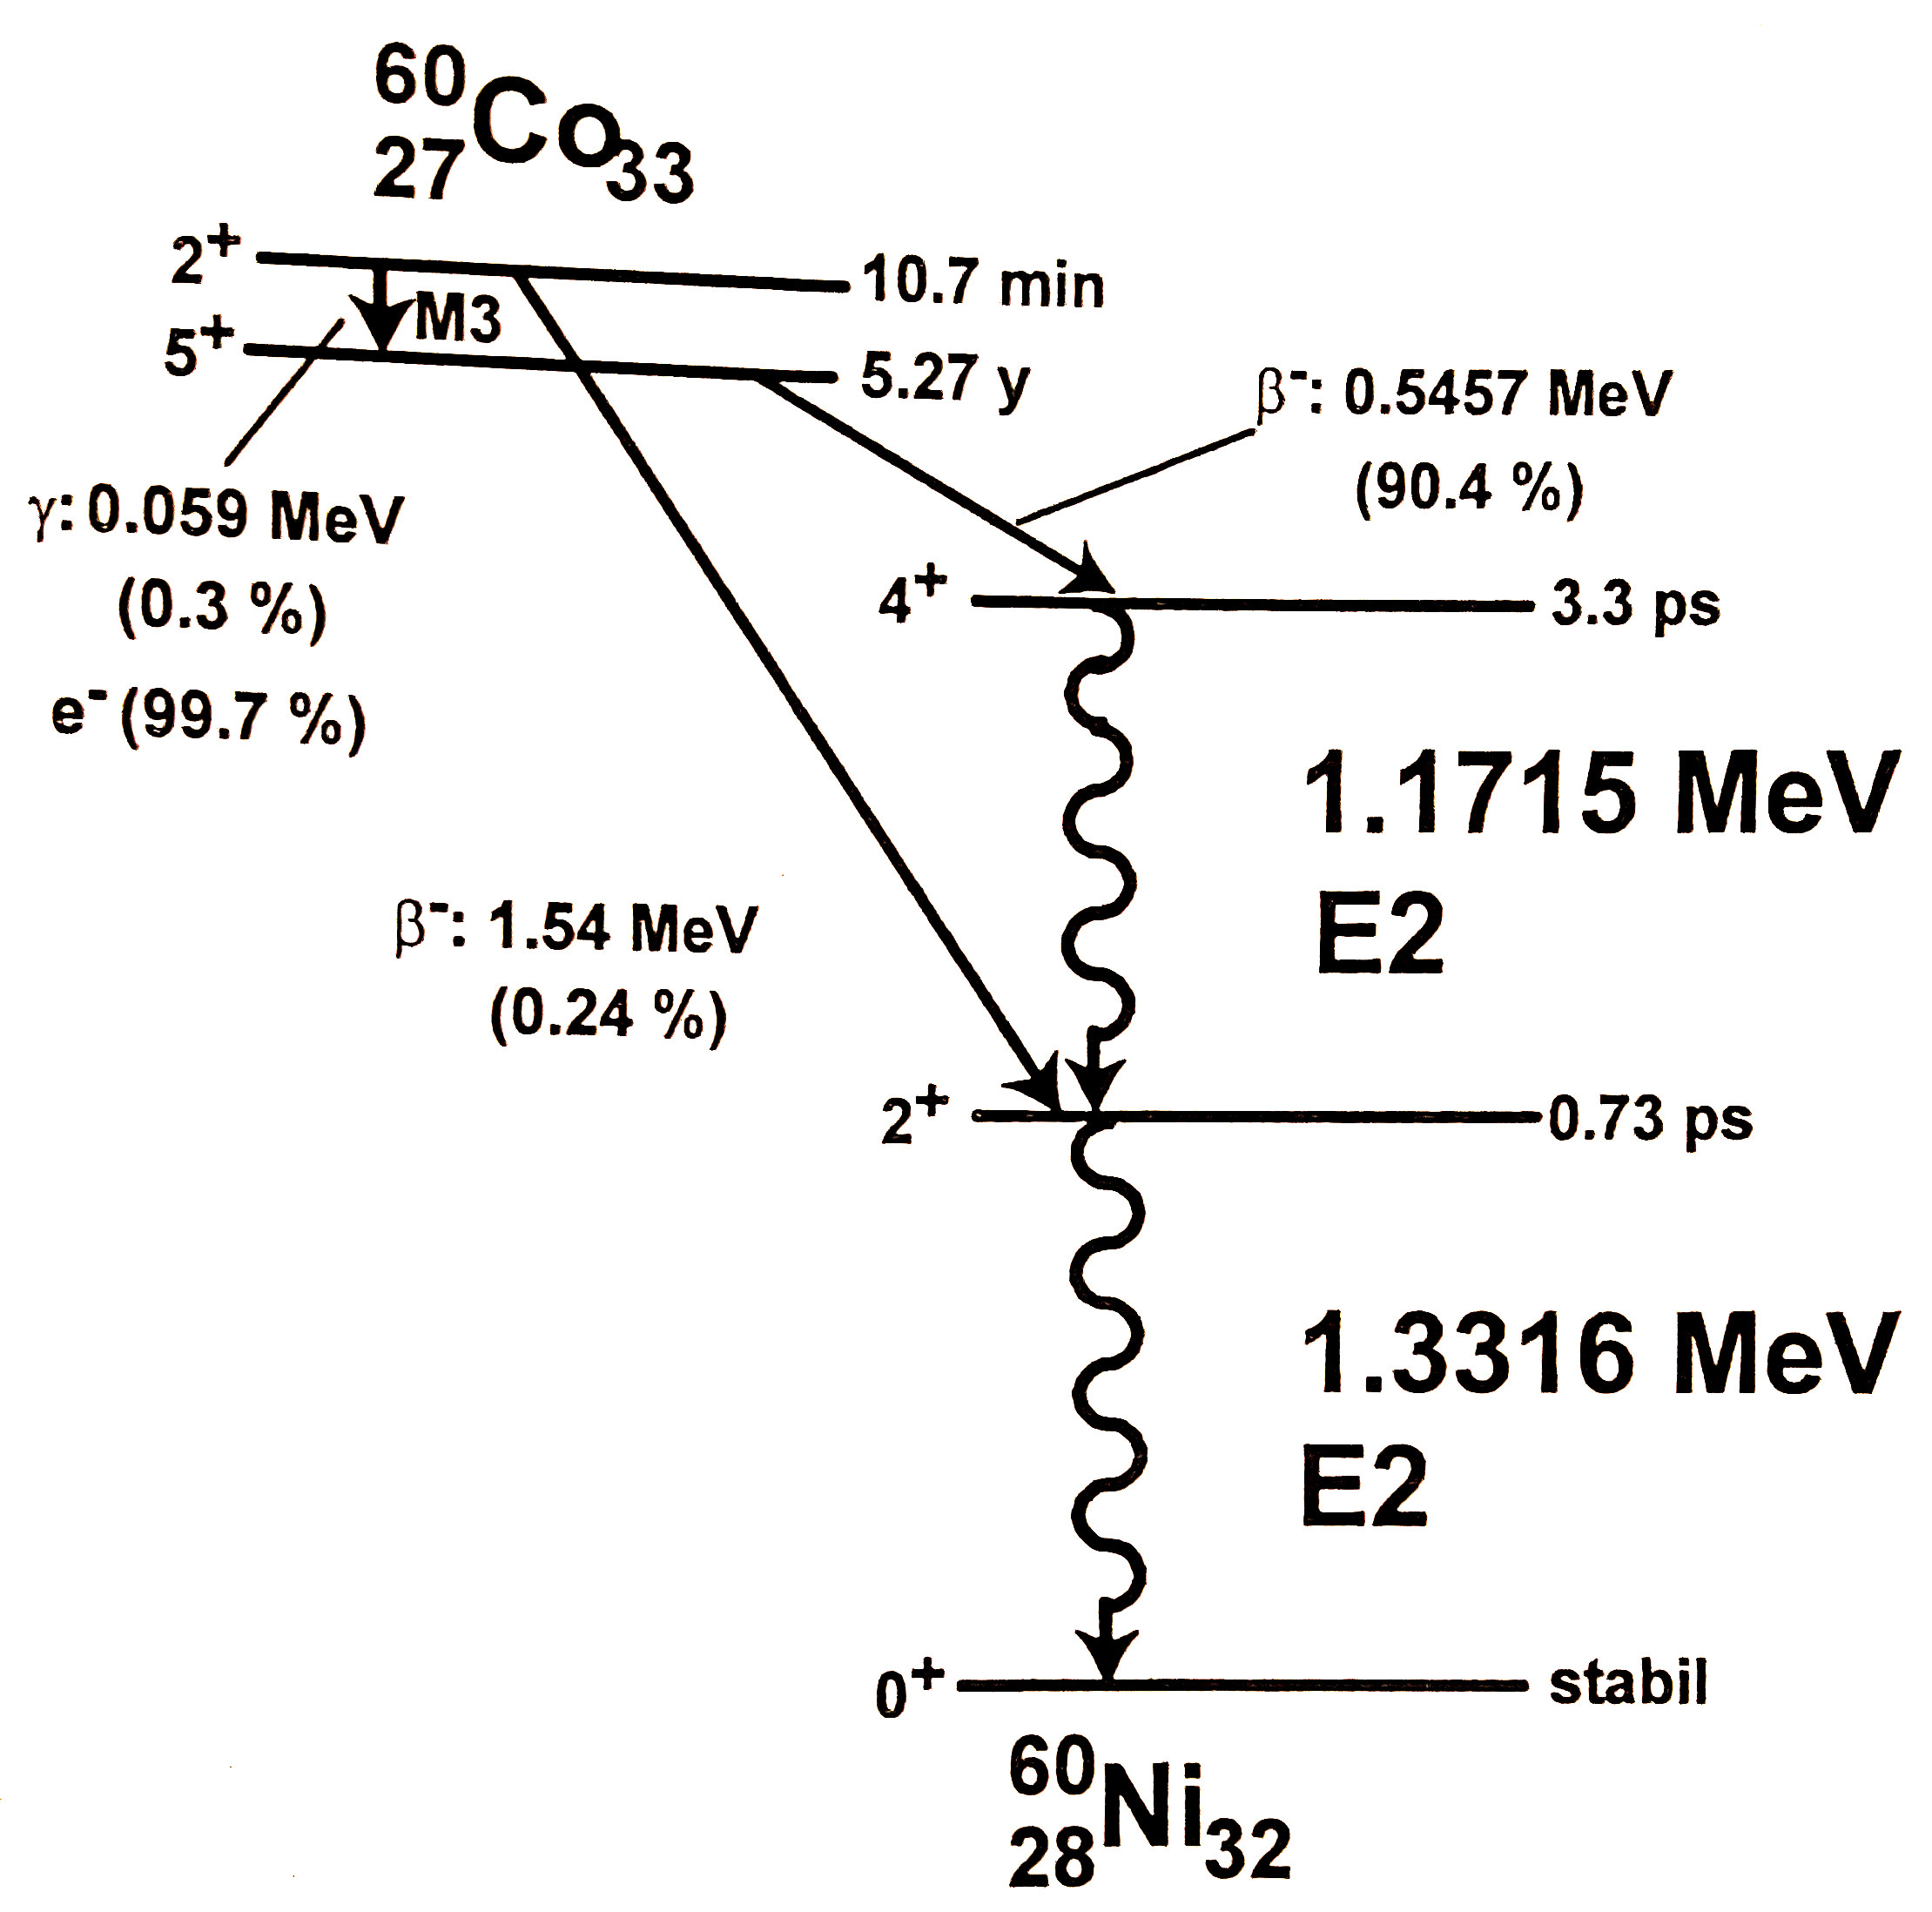
\includegraphics[width=\textwidth]{img/ZerfallsschemaVonCo60}
		\caption{Zerfallsschema von $^{60}$Co.}
	\end{subfigure}
	\caption{Die Abbildung zeigt die Zerfallsschemata der drei Strahlungsquellen Natrium-$22$, Caesium-$137$ und Cobalt-$60$. Die drei Zerfallsschemata stammen aus Seite $10$, $19$ und $22$ der Versuchsanleitung\cite{wwu}.}
	\label{Zerfallsschemata}
\end{figure}
\noindent Die NaJ-Detektoren werden so um eine Strahlungsquelle platziert, dass sie auf diese gerichtet sind.
Beide sind um die Position der Strahlungsquelle drehbar, sodass sich zwischen ihnen ein Winkel $\theta$ einstellen lässt.
Die NaJ-Detektoren setzen sich aus einem anorganischen Szintillationskristall (Natriumjodid) und einem mit dem Kristall optisch gekoppelten Photomultiplier zusammen.
Letztere besitzen einen zur Signalformung in die Basis integrierten Emitterfolger und werden mit Hochspannung betrieben.
Darüber hinaus sind die Photomultiplier jeweils an einen Hauptverstärker angeschlossen.
Die Hauptverstärker sind wiederum jeweils mit einem TSCA (engl. \emph{Timing Single Channel Analyzer}) verbunden.
Beide TSCA sind an dieselbe Koinzidenzeinheit angeschlossen.
Diese ist über einen ADC (engl. \emph{analog-to-digital converter}) mit dem Computer verbunden, welcher über eine entsprechende Datenaufnahme-Software verfügt und somit den Zähler bildet.

\subsection{Elektronik}

Registriert ein NaJ-Detektor ein Photon, so entsteht am Photomultiplier der im Oszilloskopbild \ref{SignalNachPhotomultiplier} dargestellte unipolare Puls.
\begin{figure}[H]
	\centering
	\begin{subfigure}[t]{0.495\textwidth}
		\centering
		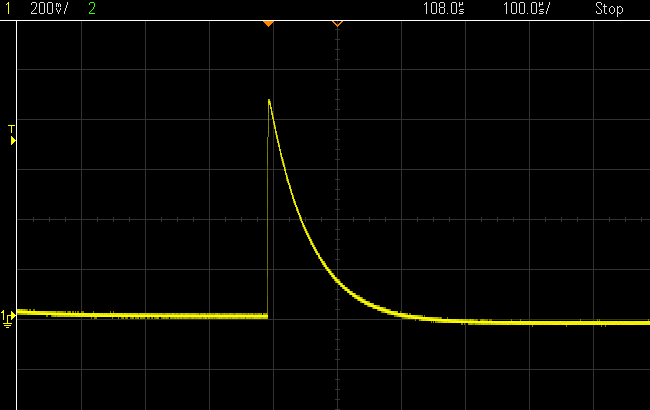
\includegraphics[width=\textwidth]{img/SignalNachPhotomultiplier}
		\caption{Oszilloskopbild des Signals aus dem Photomultiplier.}
		\label{SignalNachPhotomultiplier}
	\end{subfigure}
	\begin{subfigure}[t]{0.495\textwidth}
		\centering
		\includegraphics[width=\textwidth]{img/SignalNachHauptverstärker}
		\caption{Oszilloskopbild des Signals nach dem Hauptverstärker.}
		\label{SignalNachHauptverstärker}
	\end{subfigure}
	\begin{subfigure}[t]{0.495\textwidth}
		\centering
		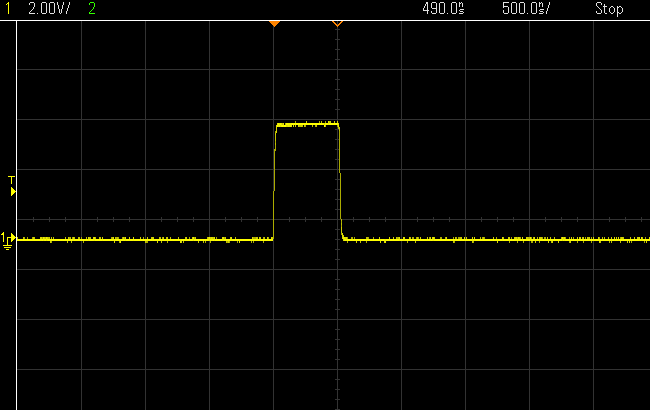
\includegraphics[width=\textwidth]{img/SignalNachTSCA}
		\caption{Oszilloskopbild des (Rechteck-)Signals nach dem TSCA.}
		\label{SignalNachTSCA}
	\end{subfigure}
	\begin{subfigure}[t]{0.495\textwidth}
		\centering
		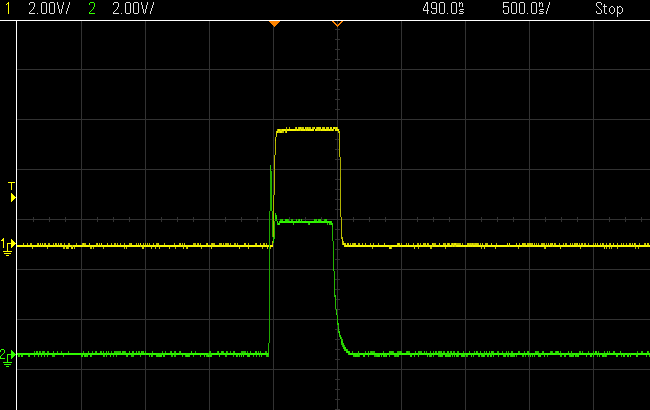
\includegraphics[width=\textwidth]{img/BeideSignaleVorKoinzidenzeinheit}
		\caption{Oszilloskopbild beider aus den TSCA stammenden (Rechteck-)Signale vor der Koinzidenzeinheit. Hierbei ist die Verzögerungszeit an einem der beiden TSCA so gewählt, dass sich beide (Rechteck-)Signale überlappen. Der beim grün markierten (Rechteck-)Signal erkennbare Einschwingvorgang ist darauf zurückzuführen, dass kein Abschlusswiderstand am Eingang des Oszilloskops angebracht wurde.}
		\label{BeideSignaleVorKoinzidenzeinheit}
	\end{subfigure}
	\caption{Die Abbildung zeigt die mit einem Oszilloskop aufgenommenen Bilder des Signals bzw. der Signale an vier verschiedenen Stellen im Blockschaltbild, welches in Abbildung \ref{schaltung} zu sehen ist.}
	\label{Oszilloskopbilder}
\end{figure}
\noindent Die Höhe der Amplitude dieses Pulses ist proportional zur im Szintillator deponierten Energie.

Der Hauptverstärker wandelt die unipolaren in bipolare Signale um, indem er sie differenziert.
Das Oszilloskopbild \ref{SignalNachHauptverstärker} zeigt solch ein bipolares Signal nach dem Verlassen des Hauptverstärkers.
Überschreitet der positive Teil des bipolaren Pulses eine gewisse Schwelle, so wird der Puls gezählt, sobald er wieder Null erreicht.
Dies entspricht immer dem Maximum des ursprünglichen, nicht-differenzierten Signals.
Somit liefert der Nulldurchgang des bipolaren Signals die eindeutige Zeitinformation und der Zeitnullpunkt ist von der Höhe der Amplitude unabhängig.

Der TSCA registriert die vom Hauptverstärker ausgehenden bipolaren Pulse und gibt Rechteckpulse aus, was im Oszilloskopbild \ref{SignalNachTSCA} zu sehen ist.
Der TSCA besitzt eine untere und eine obere Schwelle, sodass Signale, deren Höhe oberhalb der unteren und unterhalb der oberen Schwelle liegt, zu einem Rechteckpuls am Ausgang des TSCA führen.
Sobald es beim Signal am Eingang des TSCA zum Nulldurchgang kommt, beginnt der Rechteckpuls.
Zusätzlich bietet der TSCA die Möglichkeit mit Hilfe eines eingebauten Verzögerungsglieds (Delay) ein Signal zu verzögern.
Diese Verzögerungsglieder dienen dem künstlichen Ausgleich der Verzögerung von Signalen, welche zwar zeitlich gegeneinander verschobenen, aber eigentlich koinzident sind.
Die besagte Signalverzögerung kommt aufgrund der unterschiedlichen Kabellängen und der elektronischen Verarbeitungszeit in den verschiedenen Komponenten zustande.

Bei der Koinzidenzeinheit handelt es sich um eine \glqq Fast-Coincidence-Unit\grqq .
Das vor der Koinzidenzeinheit aufgenommene Oszilloskopbild \ref{BeideSignaleVorKoinzidenzeinheit} zeigt zwei von den TSCA ausgehende (Rechteck-)Signale.
Überlappen sich zwei solcher Rechteckpulse, was im Oszilloskopbild \ref{BeideSignaleVorKoinzidenzeinheit} der Fall ist, werden sie von der Koinzidenzeinheit als koinzident angesehen und es wird ein Signal an den Zähler weitergegeben.
Bei einer Koinzidenzeinheit wird auf die Flanke der Rechteckpulse getriggert und die (Rechteck-)Signale werden so umgeformt, dass die ansteigenden Flanken zu Pulsen werden.
Sobald sich diese Pulse überlappen, werden die aus den TSCA stammenden (Rechteck-)Signale als koinzident bewertet.
Anzumerken ist, dass wenn die Verzögerungszeit zwischen den aus den TSCA stammenden Signalen variiert wird, sich durch die Signalumformung ein gaußartiger Zusammenhang zwischen Verzögerungszeit und Zählrate ergibt.

Der Zähler besitzt die Aufgabe, die von der Koinzidenzeinheit registrierten Koinzidenzen zu zählen.

\subsection{Durchführung}

Um sicherzustellen, dass wahrhaftig koinzidente Signale zeitgleich an der Koinzidenzeinheit ankommen, wird bei der Versuchsdurchführung zunächst die Verzögerungsdauer bzw. -zeit (Delay) mit Hilfe der $^{22}$Na-Quelle experimentell bestimmt.
Dazu wird die Tatsache ausgenutzt, dass bei der Annihilation der von Natrium-$22$ ausgestrahlten Positronen mit den Elektronen der Aluminiumhülle der Quelle zwei koinzidente Photonen unter einem Winkel von $180\,$° ausgesendet werden.
Dementsprechend wird der Winkel zwischen den NaJ-Detektoren auf $\theta =180\,$° eingestellt.
Dadurch können die NaJ-Detektoren koinzidente Signale aus der Elektron-Positron-Vernichtung in Form von Photonen messen.
Damit die Koinzidenzeinheit diese auch als koinzidente Ereignisse erkennt, wird eines der beiden Verzögerungsglieder am TSCA schrittweise verstellt.
Bei jeder der dadurch entstehenden Verzögerungen in der entsprechenden Signalleitung wird $30$ Sekunden lang die Anzahl der Koinzidenzen gemessen.
Auf diese Weise wird eine Reihe von Verzögerungszeiten durchgetestet.
Die Verzögerungszeit, welche die höchste Zählrate liefert, wird im weiteren Verlauf des Experiments verwendet.
Es ist zu erwähnen, dass zufällige Koinzidenzen, also Einzelprozesse, welche zufällig gleichzeitig ablaufen, aber nicht miteinander korreliert sind, gegenüber den tatsächlichen Koinzidenzen unterdrückt sind.

Nun wird die $^{22}$Na-Quelle aus der Versuchsanordnung herausgenommen und gegen die $^{137}$Cs-Quelle ausgetauscht, um die Koinzidenzauflösungszeit $2\tau$ zu ermitteln.
Dazu wird für jeden einzelnen NaJ-Detektor zwei Minuten lang die Zählrate gemessen.
Anschließend werden die Koinzidenzen $30$ Minuten lang bei einem Winkel von $\theta =120\,$° gemessen.
Caesium-$137$ wird als Quelle verwendet, weil der im Zuge des $\beta^{-}$-Zerfalls entstehende angeregte Kernzustand von Barium-$137$ beim $\gamma$-Zerfall ein Photon emittiert.
Dies ist anhand des Zerfallsschemas von $^{137}$Cs in Abbildung \ref{Zerfallsschemata} nachzuvollziehen.

Die $^{137}$Cs-Quelle wird aus der Versuchsanordnung herausgenommen und wieder gegen die $^{22}$Na-Quelle ausgetauscht, sodass die Winkelkorrelation der Vernichtungsstrahlung untersucht werden kann.
Zunächst wird für jeden einzelnen NaJ-Detektor zwei Minuten lang die Zählrate gemessen.
Anschließend werden bei $\theta =90\,$° und $\theta =120\,$° jeweils $10$ Minuten lang die Koinzidenzen gemessen.
Hierbei handelt es sich um zufällige Koinzidenzen.
Nun wird der Winkel $\theta$ von $170\,$° bis $190\,$° in $2\,$°-Schritten variiert, wobei jeweils drei Minuten lang die Koinzidenzen gemessen werden.

Zuletzt wird die $^{22}$Na-Quelle wieder aus der Versuchsanordnung herausgenommen und die $^{60}$Co-Quelle eingesetzt, um die Winkelkorrelation der $\gamma$-$\gamma$-Kaskade von Cobalt-$60$ zu untersuchen.
Dazu wird für jeden einzelnen NaJ-Detektor zwei Minuten lang die Zählrate gemessen.
Anschließend wird bei $\theta =90\,$° und $\theta =180\,$° jeweils $30$ Minuten lang die Anzahl der Koinzidenzen registriert.
Zur Bestimmung der zufälligen Koinzidenzen wird eines der Verzögerungsglieder bis zum Anschlag herausgedreht, sodass die Messung von tatsächlichen Koinzidenzen vermieden wird.